% LaTeX Template for short student reports.
% Citations should be in bibtex format and go in references.bib
\documentclass[a4paper, 11pt]{article}
\usepackage[top=3cm, bottom=3cm, left = 2.5cm, right = 3cm]{geometry}
\usepackage[english]{babel} 
\geometry{a4paper} 
\usepackage[utf8]{inputenc}
\usepackage{textcomp}
\usepackage{graphicx} 
\usepackage{amsmath,amssymb} 
\usepackage{mathtools} 
\usepackage{bm}  
\usepackage[hidelinks]{hyperref} 
\usepackage{float}
\usepackage{algpseudocode}
\usepackage{algorithm}
\usepackage{parskip}

\usepackage{setspace}
\onehalfspacing

\usepackage{pgfplots}
\pgfplotsset{width=10cm,compat=1.9}

% \setlength{\parindent}{0cm}
%\hypersetup{linkcolor=black,citecolor=black,filecolor=black,urlcolor=black} % black links, for printed output
\usepackage{memhfixc} 
\usepackage{pdfsync}  
\usepackage{fancyhdr}
\pagestyle{fancy}

\usepackage[compact]{titlesec}  
\titlespacing*{\section}{0pt}{10ex plus 1ex minus .2ex}{4.3ex plus .2ex}

\usepackage[backend=biber, maxbibnames=99]{biblatex}


\usepackage{amsthm}


\newtheorem*{example*}{Example}
\newtheorem*{definition*}{Definition}




\addbibresource{references.bib}

\title{Runtime analysis of the Java implementation of the CYK-algorithm}
\author{Pina Kolling \\ piko0011@student.umu.se}
%\date{}


\newcommand{\dq}{"}






%---------------------------------------------------------------------%

%---------------------------------------------------------------------%






\begin{document}


\begin{titlepage}
	\centering
	{\scshape\LARGE Ume\r{a} University \par}
	Efficient Algorithms \par
	\vspace{1cm}
	{\scshape\Large Assignment Step 2 \par }
	\vspace{1.5cm}
	{\huge\bfseries  Runtime analysis of the Java implementation of the CYK-algorithm \par}
	\vspace{2cm}
	{\Large\itshape Pina Kolling\par}
	\vfill

% Bottom of the page
	{\large \today\par}
\end{titlepage}








%---------------------------------------------------------------------%







\setcounter{page}{1}


\newpage
\fancyhead[LO]{\empty}
{
  \hypersetup{linkcolor=black}
  \tableofcontents
}




\newpage





%---------------------------------------------------------------------%








\section{Introduction}

Parsing in Computer Science is the process  of reading and processing an input. In this context it is used for analysing a string of characters to examine if the string is built according to the rules of a formal grammar. 

A formal grammar describes how to form strings with correct syntax out of characters from a formal language's alphabet (explained in section \ref{formalgrammar} and \ref{formallanguage}).
To examine if such a string follows the rules of a grammar, the \textit{Cocke-Younger-Kasami}-algorithm (short: \textit{CYK}) can be used. This algorithm is described in section \ref{cyk}. To use the \textit{CYK}-algorithm the grammar needs to be in a specific format, that is called \textit{Chomsky-Normal-Form} (short: \textit{CNF}), which is explained in section \ref{cnf}. \cite{CYK_name, CYK1}


The task for this assignment is to code three different parsing methods of which one executes the \textit{CYK}-algorithm with dynamic programming in \textit{Java}. The different parsing methods will be described and presented as pseudo code in section \ref{systemdesign}.
For the implementation three different classes are implemented: \texttt{main.java, grammar.java} and \texttt{parser.java}. The \texttt{main}-class calls the methods and the \texttt{grammar}-class parses the input grammer as string into a format that then can be processed in the \texttt{parser}-class. This \texttt{parser}-class has three different parsing methods, which will be tested and compared against each other.
The function and implementation will be former described in section \ref{systemdesign}. Also in section \ref{systemdesign} the runtimes in $O$-notation are calculated for each approach.


In section \ref{evaluation} the runtimes and experiments of the different algorithms are compared and differences in efficiency are shown.

In the final part (section \ref{conclusion}) the results and future possibilities are discussed.




\pagebreak






%---------------------------------------------------------------------%








\section{Background}

In this section background information, definitions and examples on formal languages, alphabets and Kleene star (section \ref{formallanguage}), formal grammars (section \ref{formalgrammar}), Chomsky-Normal-Form (section \ref{cnf}), CYK-algorithm (section \ref{cyk}) and dynmaic programming (section \ref{dp}) will be presented. 

%---------------------------------------------------------------------%

\subsection{Formal language}
\label{formallanguage}


Formal languages are abstract languages, which define the syntax of the words that get accepted by that language. It is a set of words that get accepted by the language and has a set of symbols that is called alphabet, which contains all the possible characters of the words. Those characters are called nonterminal symbols. \cite{CNF, language}

\begin{definition*}[Kleene star]
The Kleene star $\Sigma^*$ of an alphabet $\Sigma$ is the set of all words that can be created through concatenation of the symbols of the alphabet $\Sigma$. The empty word $\epsilon$ is included. 
\end{definition*}

\begin{definition*}[Formal language]
A formal language $L$ over an alphabet $\Sigma$ is a subset of the Kleene star of the alphabet: $L \subseteq \Sigma^*$
\end{definition*}


\begin{example*}[Formal language]\footnote{The following examples show the \textit{Well-Balanced Parantheses} example from the assignment task sheet with the alphabet $\{a, b\}$ instead of $\{(, )\}$. } The language accepts words that contain the same number of $a$s and $b$s, while the a has to be left of the b. 
The alphabet $\Sigma$ of this language looks like this:
\begin{align*}
\Sigma & = \{ a, b\}
\end{align*}
The Kleene star $\Sigma^*$ of the alphabet $\Sigma$ looks like this:
\begin{align*}
\Sigma^* & = \{ \epsilon, a, b, aa, ab, ba, bb, aaa, aab, abb, bbb, bba, baa, aba, bab, ...   \}
\end{align*}
The language definition $L$ is the following one:
\begin{align*}
L = \{ (a^{n}b^{n})^m \} \text{ with } n, m \in \mathbb{N}
\end{align*}

\end{example*}



%---------------------------------------------------------------------%

\subsection{Formal grammar}
\label{formalgrammar}


A formal grammar describes how to form strings with correct syntax from a language's alphabet. A grammar does not describe the meaning of the strings or any semantics — only their syntax is defined. The grammar is a set of rules, which define which words are accepted by a formal language. Those rules consist of terminal and nonterminal symbols. The terminalsymbols are the characters of the alphabet of the language and the nonterminalsymbols are used to build the rules of the language -- they get replaced by terminalsymbols. \cite{CNF, language} 

\begin{definition*}[Formal grammar]
A formal grammar $G$ is defined as a 4-tuple:
\begin{align*}
G = (V, T, P, S)
\end{align*}
The set $V$ contains the nonterminal symbols of the grammar and the set $T$ the terminal symbols, which is the alphabet of a language. This assumes that $V \cap T = \emptyset$. The set $P$ is the set of production rules, where an element of $V$ points to an element of $V^* \times T^*$. The symbol $S \in V$ represents the start symbol. 

The production rules in the set $P$ have the format $head \rightarrow body$. The head is always a nonterminal symbol and the body can be a combination of terminal and nonterminal symbols. A nonterminal symbol $A$ in the body of a rule can be replaced by the body of a rule with the form $A \rightarrow body$.
\cite{LS_Ulm}
\end{definition*}

\begin{example*}[Formal grammar]
The example grammar $G$ for the previous example language $L$ over the alphabet $\Sigma$ is the following:
\begin{align*}
G = (\{S\}, \{ a, b \}, \{ S \rightarrow SS, S \rightarrow  aSb, S \rightarrow ab \},  \{ S \})
\end{align*}
The rules of the grammar $G$ over the alphabet $\{a, b\}$ with the start symbol $S$ and the nonterminal symbols $\{ S \}$ can also be written in the following form:
\begin{center}
\texttt{S $\rightarrow$ SS $\mid$  aSb $\mid$ ab}
\end{center}
\end{example*}

%---------------------------------------------------------------------%

\subsection{Chomsky-Normal-Form}
\label{cnf}

The \textit{Chomsky-Normal-Form} (short: \textit{CNF}) is a grammar which is formated in a specific way. If the head of a rule (nonterminal symbol) is not generating the empty word (\textit{\texttt{S $\rightarrow \epsilon$}}) it either generates two nonterminal symbols or one terminal symbol for the grammar to be in \textit{CNF}.
\cite{CNF}

\begin{example*}[Chomsky-Normal-Form]
This is the previous example in CNF. How it was built can be seen in appendix \ref{createcnf}.
\begin{align*}
\texttt{S} & \rightarrow \texttt{SS} \mid  \texttt{LA} \mid \texttt{LR} \\
\texttt{A} & \rightarrow \texttt{SR} \\
\texttt{L} & \rightarrow a \\
\texttt{R} & \rightarrow b
\end{align*}
\end{example*}


%---------------------------------------------------------------------%

\subsection{CYK-algorithm}
\label{cyk}


\textit{Cocke-Younger-Kasami}-algorithm (short: \textit{CYK}-algorithm) takes a grammar $G = (V, T, P, S)$ in \textit{CNF} and a word $w= w_1, w_2, ..., w_n \in T^*$ as an input. It then examines if the word follows the rules of the grammar. Then for every substring $w_{i, j} = w_i, ..., w_{i+j-1}$ (begins at index $i$ and has the length $j$) of the word $w$  the set of nonterminal symbols that lead to $w_{i, j}$ gets calculated and saved as $V_{i, j}$ to access it in later steps. \cite{CYK1}


\begin{example*}[Chomsky-Normal-Form]
The following table shows the CYK-algorithm with the previous grammar example and the input word $aaabbb$. \cite{cyk_online_alg}
\begin{figure}[H]
\begin{center}
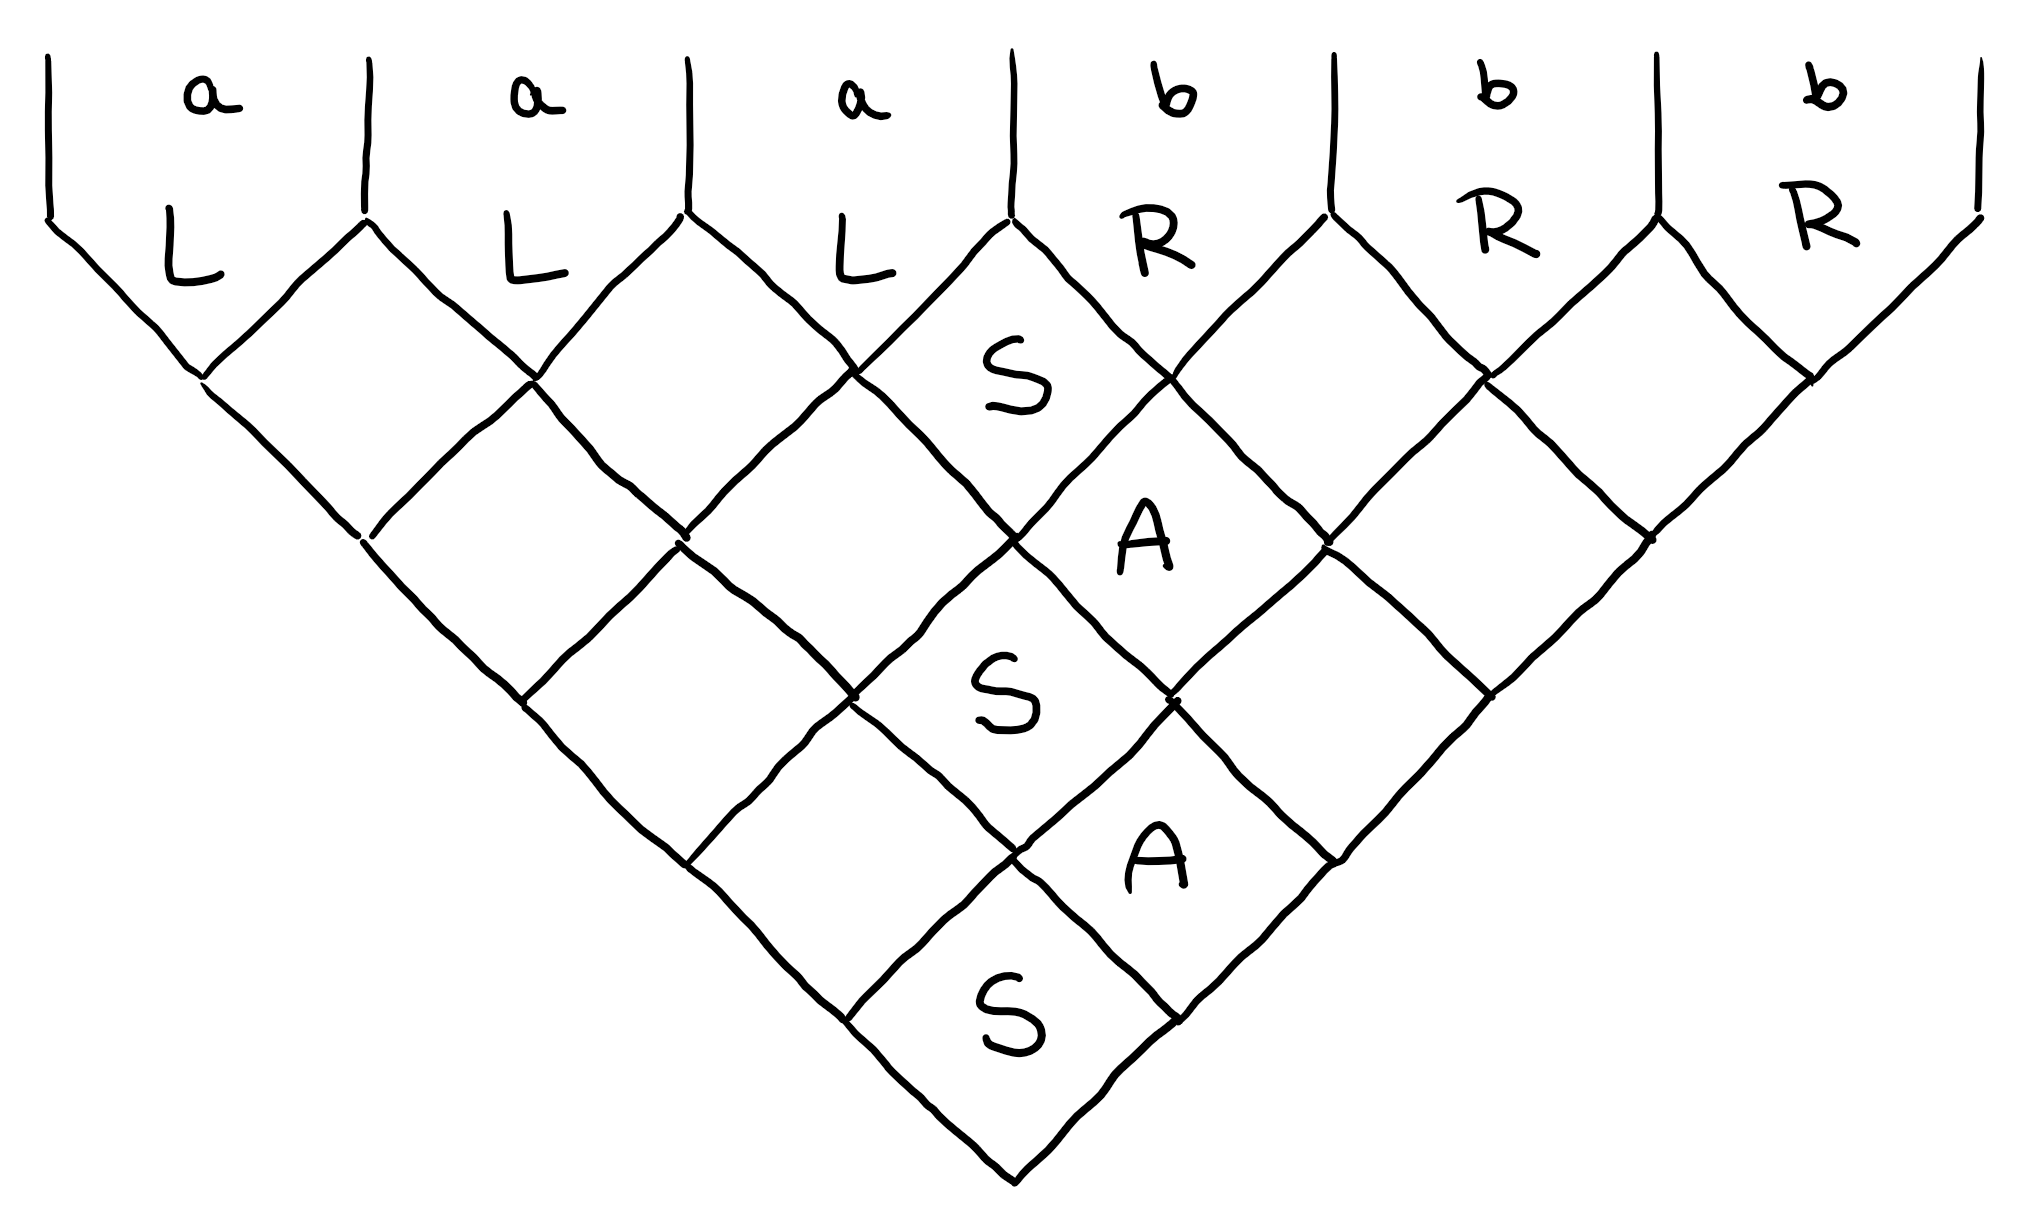
\includegraphics[scale=0.3]{images/cyk_table.png}
\end{center}
\caption{CYK-algorithm table for the word $aaabbb$}
\end{figure}
The word is accepted by the grammar rules, because the intiating nonterminal symbol \textit{\texttt{S}} can be filled into the lowest field. In appendix \ref{cyksteps} the table is filled in step by step and the rules that are used in each step are marked, for a better understanding on how the algorithm works.
\end{example*}

%---------------------------------------------------------------------%

\subsection{Dynamic programming}
\label{dp}

The technique of dynamic programming can be used to solve problems, which can be devided into smaller subproblems. The solutions of the subproblems are saved (for example in a multi-dimensional array) and referenced later. \cite{DP}
\\
\begin{example*}[Knapsack problem]

As an example the table for the knapsack problem is filled out, because it is a really common example for the concept of dynamic programming.
\\ \\
Given is a set of items with a weight and a value. The task is to choose which items to include so that the total weight is less than the given limit of the knapsack and the total value is as large as possible.
\\ \\
The formula with which the dynamic programming works is the follwing:

  
  \ \\
  $$
Opt(i,j)=
\begin{cases}
0, & \text{for } 0\leq j \leq size\\
        Opt(i-1, j), & \text{for } j < w[i]\\
        max\{ Opt(i-1, j), v[i]+Opt(i-1, j-w[i]) \}, & \text{else } 
\end{cases}
$$
\ \\

If $0 \leq j \leq w$ then there are no objects which could be put into the bag. The second case acts when object $i$ does not fit into the bag and the optimal solution is found with the objects from index $1$ to $i-1$. Else the object $i$ is either part of the optimal solution or it consists out of the objects $1$ to $i-1$.

\ \\

The table of the values and weight of each item with index $i$ is shown on the left and on the right is the table that gets filled in with a dynamic programming approach of the formula above. The maximum bag size is 7.
\\ \\
\begin{minipage}{0.3\textwidth}

\begin{tabular}{|c|c|c|}
\hline
$i$ & $w[i]$ & $v[i]$ \\
\hline
1 & 1 & 1 \\
2 & 3 & 4 \\
3 & 2 & 3 \\
4 & 4 & 6 \\
5 & 6 & 8 \\
\hline
\end{tabular}


\end{minipage}\begin{minipage}{0.1\textwidth}
\ 
\end{minipage}\begin{minipage}{0.6\textwidth}

\begin{tabular}{|c||c|c|c|c|c|c|c|c|}
\hline
5 & 0 & 1 & 3 & 4 & 6 & 7 & 9 & 10 \\
\hline
4 & 0 & 1 & 3 & 4 & 6 & 7 & 9 & 10 \\
\hline
3 & 0 & 1 & 3 & 4 & 5 & 7 & 8 & 8 \\
\hline
2 & 0 & 1 & 1 & 4 & 5 & 5 & 5 & 5 \\
\hline
1 & 0 & 1 & 1 & 1 & 1 & 1 & 1 & 1 \\
\hline
0 & 0 & 0 & 0 & 0 & 0 & 0 & 0 & 0 \\
\hline
\hline
  & 0 & 1 & 2 & 3 & 4 & 5 & 6 & 7 \\
\hline

\end{tabular}

\end{minipage}

\ \\

The first column in the table represent the objects and the last row the weight. The entries in the table show the maximum value. In this example the maximum value for the size 7 is 10.


\end{example*}







%---------------------------------------------------------------------%



\pagebreak





%---------------------------------------------------------------------%








\section{System Design}
\label{systemdesign}

The implementation was done in Java and three different classes were implemented: \texttt{main.java} (described in section \ref{main}), \texttt{grammar.java} (described in section \ref{grammar}) and \texttt{parser.java} (described in section \ref{parser}). The \texttt{main}-class calls the methods and the \texttt{grammar}-class parses the input grammer ans string into a format that then can be processed in the \texttt{parser}-class.


%---------------------------------------------------------------------%



\subsection{Main}
\label{main}

The \texttt{main}-class takes the input grammar and word and parses them into \texttt{String[]} and \texttt{String}. The arguments have to follow the following rules:
\begin{itemize}
\item The Grammar needs to be in \textit{CNF}.
\item The first rule begins with the start symbol of the grammar.
\item The rules are put in wothout arrows, one rule body is represented by one string, beginning with the rule head.
\item The last argument is the input word.
\end{itemize}
Input example (\textit{Well-Balanced-Parantheses}):\\
  \texttt{java Main \dq SSS\dq \ \dq SLA\dq \ \dq SLR\dq \ \dq ASR\dq \ \dq L(\dq \ \dq R)\dq\  \dq (())\dq}
\\ 
for the grammar \texttt{S $\rightarrow$ SS | LA | LR, A $\rightarrow$ SR, L $\rightarrow$ (, R $\rightarrow$ )} and the input word \texttt{(())}. \\
A more detailed description on how to run the code can be found in appendix \ref{howtousethecode}.


%---------------------------------------------------------------------%
%---------------------------------------------------------------------%

\subsection{Grammar}
\label{grammar}



\begin{minipage}{0.6\textwidth}
\vspace*{-2em}

The \texttt{grammar}-class assigns the nonterminal symbols to integers and builds arrays with them. The start symbol for example is then assigned with the integer zero and the bodies of that rule are at the index zero of an two-dimensional array. One array that only contains nonterminal symbols is build, one array that contains terminal and nonterminal symbold and one array that represents the integers that represent each nonterminal symbol is built.

For the input \texttt{java Main \dq SSS\dq \ \dq SLA\dq \ \dq SLR\dq \ \dq ASR\dq \ \dq L(\dq \ \dq R)\dq\  \dq (())\dq} the two-dimensional arrays shown on the screenshot on the right side are built.

(Right now the arrays still have the type \texttt{String[][]}, that will be changed later to \texttt{int[][][]} to minimize the access time in the parsing methods.)


\end{minipage}\begin{minipage}{0.1\textwidth}
\ 
\end{minipage}\begin{minipage}{0.3\textwidth}
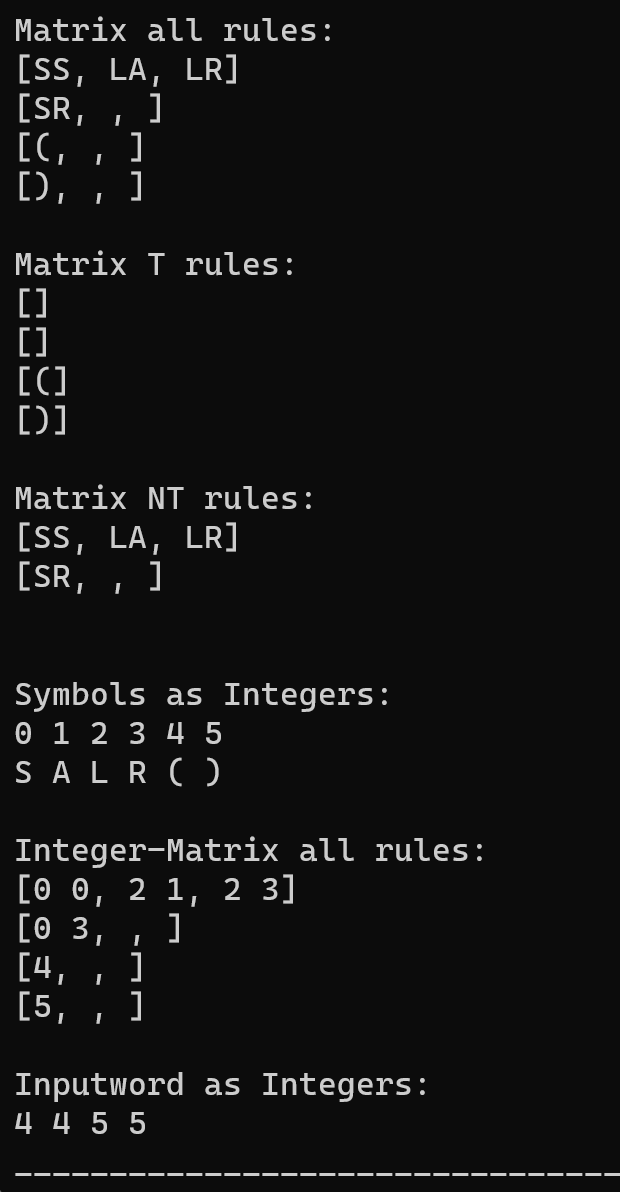
\includegraphics[scale=0.6]{images/terminal_1.png}
\end{minipage}


%---------------------------------------------------------------------%
%---------------------------------------------------------------------%

\subsection{Parser}
\label{parser}

The \texttt{parser}-class contains three different parsing methods: \texttt{parseNaive} (described in section \ref{naivedescription}), \texttt{parseTopDown} (described in section \ref{topdowndescription}) and \texttt{parseBottomUp} (described in section \ref{bottomupdescription}). Each methods has a counter as \texttt{long} which counts the number of interations and a timer as \texttt{long} in $ms$ which measures the runtime of the method. In the following sections the algorithms are described, presented as pseudo code and the runtime is analysed.

%---------------------------------------------------------------------%

\subsubsection{Naive description}
\label{naivedescription}

% TODO: describe idea of algorithm more detailed in text form!

The naive algorithm is a recursive algorithm which returns a boolean and has an initial method to start the recursion with the start values:
\begin{itemize}
\item The start symbol of the grammar is first parameter. It is an integer called \texttt{indexNT} and initialized with 0, because the start symbol is assigned to the index 0.
\item The second parameter is the integer 0 as a start index of the input word.
\item The third parameter is the integer $n$, which is the length of the input word.
\end{itemize} 
The start values get assignened in the recursion call which can be seen in the following pseudo code:
 
\begin{algorithm}[H]
\label{alg_naive_rec_call}
\caption{Recursion call: Boolean parseNaive()}\label{alg:cap}
\begin{algorithmic}[1]
\State $counter \gets 0$
\State \Return parseNaive(0, 0, inputWord.length)
\end{algorithmic}
\end{algorithm}

The naive approach does not use dynamic programming. Instead it checks for each call \texttt{parseNaive(indexNT, i, j)} first if i = j-1 and checks if the nonterminal symbol head of \texttt{indexNT} leads to a body of a rule with \texttt{s[i]}. This is the base case of the recursion which then returns true or false depending if the rule \texttt{indexNT $\rightarrow$  s[i]} exists. This base case can be seen in line 2-7 in the pseudo code below.
\\ 
\\
If i is not equal to j-1 it loops for the integer $k$ from i+1 to j-1 and checks for all rules \texttt{A $\rightarrow$ BC} if both calls \texttt{parseNaive(B, i, k)} and \texttt{parseNaive(C, k, j)} return true. This recursive call applies the function on the substrings of the input word. If such a pair of substrings is found, the function returns true, because the recursive call in combination with the \grqq \texttt{and}\grqq \ leads to the result of the complete word. If such a pair cannot be found the function returns false after looping through all rule bodies and values for $k$. This part of the recursion can be seen in the pseudo code below in line 9-21.





\begin{algorithm}[H]
\label{alg_naive}
\caption{Boolean parseNaive(int indexNT, int i, int j)}\label{alg:cap}
\begin{algorithmic}[1]
\State $counter \gets counter+1$
\If{$i == (j-1)$}
\For{$l \gets 0$ \textbf{to} $ruleset[0].length$}
\If{$ruleset[indexNT][1] == inputWord[i]$}
\State \Return true
\EndIf
\EndFor

\Else
\For{$bodyIndex \gets 0$ \textbf{to} $ruleset[indexNT].length$}
\If{$ruleset[indexNT][bodyIndex].length >= 2$}
\State $first \gets ruleset[indexNT][bodyIndex].charAt(0)$
\State $second \gets ruleset[indexNT][bodyIndex].charAt(1)$
\For{$k \gets i+1$ \textbf{to} $j$}
\If{$parseNaive(first, i, k)$ \textbf{and} $parseNaive(second, k, j)$}
\State \Return true
\EndIf
\EndFor
\EndIf
\EndFor
\EndIf
\State \Return false
\end{algorithmic}
\end{algorithm}

\subsubsection{Naive runtime}
\label{naiveruntime}

In the following table the upper bound runtime of the second method (algorithm 2) is listed for each line. The variable $n$ represents the length of the input word and $k$ the dimension of the rule array.
\ \\ \ \\
\begin{minipage}{0.5\textwidth}

\begin{tabular}{|c|c|l|}
\hline
Line & Runtime & Type \\
\hline
1 &  1 & Assignment \\
2 &  1 & Comparison \\
3 & k  & Loop \\
4 & 1 $\cdot$ k & Comparison \\
5 & 1 $\cdot$ k & Return statement\\
9 & k & Loop \\
10 & 1 $\cdot$ k & comparison \\
11 & 1 $\cdot$ k & Assignment \\
12 & 1 $\cdot$ k & Assignment\\
13 & n $\cdot$ k & Loop \\
14 & n $\cdot$ n $\cdot$ k & Recusrsive call \\
15 & 1 $\cdot$ n $\cdot$ k & Return statement\\
21 & 1 & Return statement \\
\hline
\end{tabular}

\end{minipage}\begin{minipage}{0.5\textwidth}
Calculating the runtime:
\vspace*{-1em}
\begin{align*}
& 1 + 1+ k + k +k + k + k + k + k \\
& + n \cdot k + n \cdot n \cdot k + n \cdot k \\
& =  2 + 7k + 2(n \cdot k) + n \cdot n \cdot k \\
& = 2 + 7k + 2n \cdot 2k + 2n^2 \cdot k \\
& \in O(n^2)
\end{align*}
The runtime of the naive method is in $O(n^2)$.
\end{minipage}

%---------------------------------------------------------------------%


\newpage
\subsubsection{Top-Down description}
\label{topdowndescription}

% TODO: describe idea of algorithm more detailed in text form!

The top-down method is an improves version of the naive method (section \ref{naivedescription}). This algorithm works recursive, too. In this algorithm another global array is used, which contains the values \texttt{true}, \texttt{false} and \texttt{null}. The array gets intialized with \texttt{null} in each field. That happens in the recursion call method below.

\begin{algorithm}[H]
\caption{Recursion call: Boolean parseTD()}\label{alg:cap}
\begin{algorithmic}[1]
\State $counter \gets 0$
\For{$i \gets 0$ \textbf{to} $table.length$ }
\For{$j \gets 0$ \textbf{to} $table[i].length$}
\For{$k \gets 0$ \textbf{to} $table[i][j].length$}
\State $table[i][j][k] \gets null$
\EndFor
\EndFor
\EndFor
\State \Return parseTD(0, 0, inputWord.length)
\end{algorithmic}
\end{algorithm}

Additional to the naive algorithm, the recursion in the topdown approach starts with another condition: If one of the values in the global table is not \texttt{null}, the next recursive call is not executed and this value gets returned. This if-condition can be seen in the following part of the pseudo code. The rest of the topdown approach is a similar approach to the naive method that was already described in section \ref{naivedescription}.

\begin{algorithm}[H]
\caption{Additional condition in Boolean parseTD(int indexNT, int i, int j)}\label{alg:cap}
\begin{algorithmic}[1]
\If{table[indexNT][i][j] \ != null}
\State \Return table[indexNT][i][j]
\EndIf
\end{algorithmic}
\end{algorithm}

The complete topdown algorithm is shown as pseudo code below. In the inner for-loop (line 18) the boolean value of the next method calls get assigned into the global table. If there is assigned a true (line 19) the value true gets returnes (lime 20). The general topdown approach is the same approach to the naive method that was already described in section \ref{naivedescription}.

\begin{algorithm}[H]
\caption{Boolean parseTD(int indexNT, int i, int j)}\label{alg:cap}
\begin{algorithmic}[1]
\State $counter \gets counter+1$
\State $rulesetLength \gets ruleset[0].length$
\If{$table[indexNT][i][j] \  != null$}
\State \Return $table[indexNT][i][j]$
\EndIf
\If{$i == (j-1)$}
\For{$l \gets 0$ \textbf{to} $ruleset[0].length$}
\If{$ruleset[indexNT][1] == inputWord[i]$}
\State \Return true
\EndIf
\EndFor

\Else
\For{$bodyIndex \gets 0$ \textbf{to} $ruleset[indexNT].length$}
\If{$ruleset[indexNT][bodyIndex].length >= 2$}
\State $first \gets ruleset[indexNT][bodyIndex].charAt(0)$
\State $second \gets ruleset[indexNT][bodyIndex].charAt(1)$
\For{$k \gets i+1$ \textbf{to} $j$}
\State $table[indexNT][i][j] \gets (parseTD(first,i,k)$ \texttt{and} $parseTD(second,k,j))$
\If{$table[indexNT][i][j] == true$}
\State \Return true
\EndIf
\EndFor
\EndIf
\EndFor
\EndIf
\State \Return false
\end{algorithmic}
\end{algorithm}

\subsubsection{Top-Down runtime}
\label{topdownruntime}

In this part the runtime of the topdown method is calculated.
The variable $n$ represents the length of the input word and $k$ the dimension of the rule array. The first part of the calculation shows the recursion call method.

\ \\ \\
\begin{minipage}{0.5\textwidth}

\begin{tabular}{|c|c|l|}
\hline
Line & Runtime & Type \\
\hline
1 &  1 & Assignment \\
2 & k & Loop \\
3 & k $\cdot$ n & Loop \\
4 & k $\cdot$ n $\cdot$ n &  Loop\\
5 & k $\cdot$ n $\cdot$ n $\cdot$ 1 & Assignment\\
9 & ... & Function call\\
\hline
\end{tabular}


\end{minipage}\begin{minipage}{0.5\textwidth}
Calculating the runtime of the method call:
\begin{align*}
& 1 + k + k \cdot n + k \cdot n \cdot n + k \cdot n \cdot n \\
& = 1 + k + k \cdot n + 2(n^2 \cdot k) \\
& \in O(n^2)
\end{align*}
\end{minipage}
\ \\

The runtime analysis of the \texttt{parseTD} method is analog to the \texttt{parseNaive} runtime analysis. According to this the topdown algorithm has an upper bound runtime in $O(n^2)$, too.




%---------------------------------------------------------------------%

\newpage
\subsubsection{Bottom-Up description}
\label{bottomupdescription}

The \texttt{parseBU} method works with dynamic programming.
First a table $DP$ with the size $n \times n$ gets constructed (line 2) -- $n$ represents the input word length.
In the first step the integers that represent the nonterminal symbols that are head of a terminal rule get assigned (line 3 - 12). For the character at index i of the input word the value of $DP[i][i]$ gets the nonterminal symbol that leads to the character of the word.
The approach of dynamic programming calculates the smallest substrings first and saves them for the efficient processing of the next-bigger substrings.  The smallest substrings are the single characters.


\begin{algorithm}[H]
\caption{Boolean parseBU()}\label{alg:cap}
\begin{algorithmic}[1]
\State $wordlength \gets word.length$ 
\State $String[][] DP \gets new String[wordLength][wordLength]$
\For{$i \gets 0$ \textbf{to} $wordlength$}
\If{$ruleset \ contains \ word[i]$}
\State $temp \gets index of word[i] \ in \ ruleset$
\If{$DP[i][i] \ != null$}
\State $DP[i][i] \gets DP[i][i] + temp$
\Else
\State $DP[i][i] \gets + temp$
\EndIf
\EndIf
\EndFor

\For{$l \gets 0$ \textbf{to} $wordlength$}
\For{$i \gets 0$ \textbf{to} $wordlength - l$}
\State $j \gets i + l$
\For{$k \gets 0$ \textbf{to} $j$}

\For{$head \gets 0$ \textbf{to} $ruleset.length$}
\For{$body \gets 0$ \textbf{to} $ruleset[head].length$}
\State $conter \gets counter + 1$
\If{$ruleset[head][body].length >= 2$}
\State $first \gets ruleset[head][body].charAt(0)$
\State $second \gets ruleset[head][body].charAt(1)$
\If{$DP[i][k] \ contains \ first$ \textbf{and} $DP[k+1][j] \ contains \ second$}
\State $temp \gets head$
\State $DP[i][j] \gets DP[i][j] + temp$
\EndIf
\EndIf
\EndFor
\EndFor
\EndFor
\EndFor
\EndFor
\If{$DP[0][wordlength-1] \  contains \ 0$}
\State \Return true
\EndIf
\State \Return false
\end{algorithmic}
\end{algorithm}

In line 13 to 32 the \textit{CYK}-algorithm gets excecuted. It is descreibed in section \ref{cyk}. For each field the two fields \textit{leading} to it get compared, to then fill in the head of a rule that concludes into the both compared nonterminal symbols.

In the last lines (line 33-35) the last field of the $DP$-array gets checked. If it containes the start symbol of the grammar, the word is contained in the language and the algorithm returns true. Else false is returned.




\subsubsection{Bottom-Up runtime}
\label{bottomupruntime}

In the following part the upper bound runtime of the bottom up algorithm gets analysed.
The variable $n$ represents the length of the input word and $k$ the dimension of the rule array. \\

\begin{minipage}{0.6\textwidth}

\begin{tabular}{|c|c|l|}
\hline
Line & Runtime & Type \\
\hline
1 &  1 & Assignment \\
2 & 1 & Assignment \\
3 & n & Loop \\
4 &  n &  Comparison\\
5 & n  & Assignment\\
6 & n &  Comparison\\
7 & n &  Assignment \\
9 & n & Assignment \\
13 & n & Loop \\
14 & n $\cdot$ n& Loop\\
15  & n $\cdot$ n  & Assignment \\
16 & n $\cdot$ n $\cdot$ n & Loop \\
17  & n $\cdot$ n $\cdot$ n $\cdot$ k & Loop \\
18  & n $\cdot$ n $\cdot$ n $\cdot$ k $\cdot$ k & Loop \\
19 & n $\cdot$ n $\cdot$ n $\cdot$ k $\cdot$ k & Assignment\\
20 & n $\cdot$ n $\cdot$ n $\cdot$ k $\cdot$ k & Comparison\\
21 & n $\cdot$ n $\cdot$ n $\cdot$ k $\cdot$ k & Assignment\\
22& n $\cdot$ n $\cdot$ n $\cdot$ k $\cdot$ k & Assignment\\
23 & n $\cdot$ n $\cdot$ n $\cdot$ k $\cdot$ k & Comparison\\
24  & n $\cdot$ n $\cdot$ n $\cdot$ k $\cdot$ k & Assignment \\
25   & n $\cdot$ n $\cdot$ n $\cdot$ k $\cdot$ k & Assignment\\
33 & 1 & Comparison\\
34 & 1 & Return statement\\
36  & 1 &  Return statement\\
\hline
\end{tabular}


\end{minipage}\begin{minipage}{0.4\textwidth}
Calculating the runtime:
\begin{align*}
& 5 + 7n + 2n^2 + n^3 +n^3 \cdot k + 8 \cdot n^3 \cdot k^2 \\
& 5 + 7n + 2n^2 + (k+1)n^3 + 8 \cdot n^3 \cdot k^2 \\
& \in O(n^3)
\end{align*}

\end{minipage}
\ \\
The runtime of the \texttt{parseBU} method is in $O(n^3)$.


%---------------------------------------------------------------------%

\pagebreak






%---------------------------------------------------------------------%







\section{Evaluation}
\label{evaluation}

In this section the runtimes and experiments will be compared.


\subsection{Experiments}
\label{experiments}

The following tables show some tests that were run with the different parsing methods and grammars. The first of each column for the method shows the truth value that is returned (as T for true and F for false), C represents the counter and T the time in ms.
\\
\\
Well-Balanced-Parantheses: \\
\\
\begin{tabular}{|c|c||c|c|c||c|c|c||c|c|c|}
\hline
Word & Length & N & NC & NT & B & BC & BT & T & TC & TT \\
\hline
\hline
() & 2 & T & 6 & 5ms & F & 0 & 2ms & T & 6 & 1ms \\
\hline
(()) & 4 & T & 33 & 4ms & F & 84 & 3ms & T & 28 & 1ms \\
\hline
((())) & 6 & T & 212 & 6ms & F & 360 & 6ms & T & 84 & 1ms \\
\hline
(((()))) & 8 & T & 1295 & 6ms & F & 924 & 9ms & T & 190 & 1ms \\
\hline
((((())))) & 10 & T & 7666 & 9ms & F & 1872 & 11ms & T & 362 & 1ms \\
\hline
(((((((((()))))))))) & 20 & T & 51.863.993 & 1049ms & F & 15.732 & 23ms & T & 2.772 & 3ms \\
\hline
((...)) & 40 & & & & F & 127.452 & 50ms & T & 21.743 & 4ms \\
\hline
\end{tabular}

\ \\
The input word with a length of 40 did not terminate for the naive parsing in 60 minutes.

%---------------------------------------------------------------------%



\subsection{Runtimes}
\label{runtime}

% TODO plot graph of runtimes

The runtimes of the methods are calculated in section \ref{systemdesign}. The results are the following:
\ \\ \\
\begin{tabular}{|l|c|}
\hline
Method & Runtime \\
\hline
\texttt{parseNaive} & $O(n^2)$\\
\texttt{ParseTD} & $O(n^2)$ \\
\texttt{ParseBU} & $O(n^3)$\\
\hline
\end{tabular}

\ \\
Seeing those runtimes one could think that the naive and the topdown approach are equally efficient. Considering the differences in the algorithms and the results of the experiments it gets shown that this is not the case. The O-notation runtimes are the upper bounds for the runtime. 

Regarding the experiments that were run on the code, the topdown method seems to be the most efficient, followed by the bottomup method. The least efficient method is in these cases the naive approach.



% TODO: n^2 und n^3 plotten!

\pagebreak





%---------------------------------------------------------------------%








\section{Conclusion and Future Work}
\label{conclusion}


\subsection{Conclusion}


Regarding the experiments from section \ref{evaluation}, the topdown method seems to be the most efficient, followed by the bottomup method. The least efficient method is in these cases the naive approach.

Depending on the input word and the grammar the naive and the topdown approach have the same worst case runtime with $O(n^2)$. The bottomup method has the highest worst case runtime with $O(n^3)$.

These algorithms show differences in efficiency but also limits for the examination of words with the \textit{CYK}-algorithm. The amount of calls raised especially with the Well-Balanced-Parantheses language exponentially. This can also be seen in the graphs in appendix \ref{graph}.

\subsection{Future work}

Formal languages and grammars can be used in different use cases. For exampel for AI learning methods. Real languages like English can be defined as a formal language, too. But it is important to consider that formal languages only define the syntax and not the semantics. In addition to this has english a lot of rules and many exceptions. \cite{FG}

\
\\
The future work for this assignment is to change the types of the arrays from \texttt{String[][]} to \texttt{int[][][]}. In addition to this there still exists a problem in the bottomup method, which needs to be fixed. Some specific grammars and words do not return the right value. After these things work correctly, more experiments can be run and the pseudo code will be edited. Then the upper bound runtime can be calculated again and the plotted graphs can be compared to the according $O$-notation runtime.


\newpage





%---------------------------------------------------------------------%








\appendix

\section{How to use the code?}
\label{howtousethecode}

The code can be run in the terminal and input is expected as Strings in quotation marks. The grammar needs to be in CNF. The first rule begins with the startsymbol of the grammar. \\ \\
First: Rules without arrows (one rule as one String) \\
Last: The last argument is the input word
\\ 

Input example (\textit{Well-Balanced-Parantheses}):\\
  \texttt{java Main \dq SSS\dq \ \dq SLA\dq \ \dq SLR\dq \ \dq ASR\dq \ \dq L(\dq \ \dq R)\dq\  \dq (())\dq}
\\ 
for the grammar \texttt{S $\rightarrow$ SS | LA | LR, A $\rightarrow$ SR, L $\rightarrow$ (, R $\rightarrow$ )} and the input word \texttt{(())}.
\\ \\
Output example: \\
The first part of the output shows the arrays, which get generated in the \texttt{Grammar.java} class.  \\ \\
\begin{minipage}{0.6\textwidth}
\vspace*{-2em}
The first array contains all rules. \\ \\ \\

The second array contains only the terminal rules. \\ \\

The third array contains only the nonterminal rules. \\

Then it is shown which nonterminal symbols are represented by which integers. Later the nonterminal symbols can be referred to with those integers. \\ 

After this the mentioned arrays are shown again but the nonterminal symbols got replaced with the according integers.

\end{minipage}\begin{minipage}{0.2\textwidth}
\ 
\end{minipage}\begin{minipage}{0.3\textwidth}
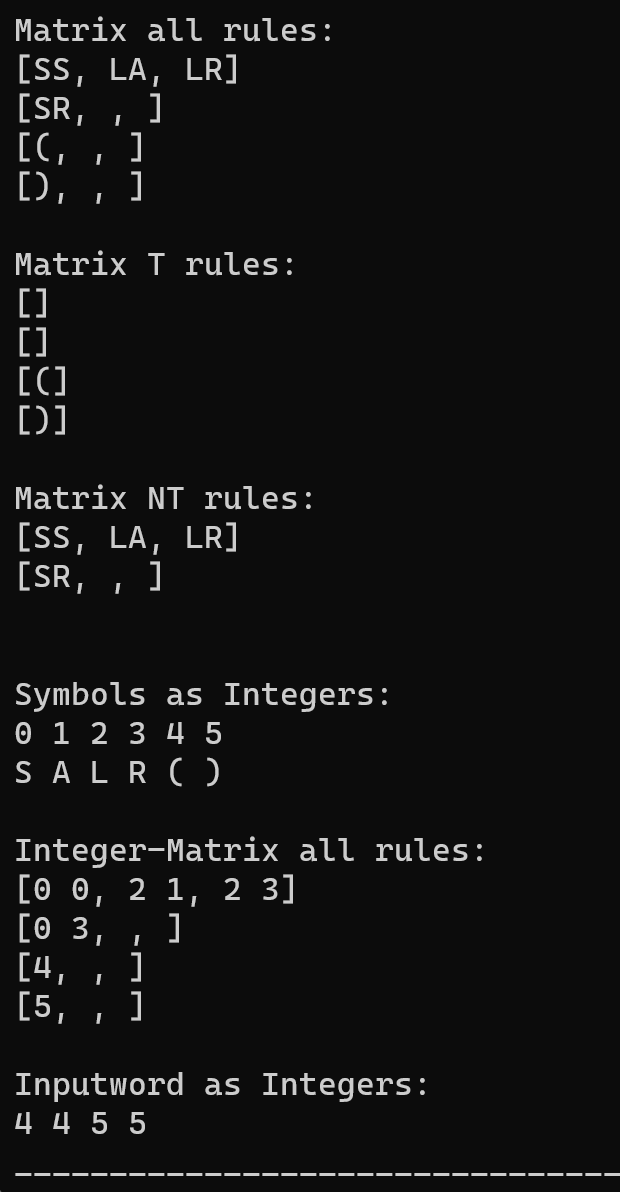
\includegraphics[scale=0.7]{images/terminal_1.png}
\end{minipage}

\begin{minipage}{0.4\textwidth}
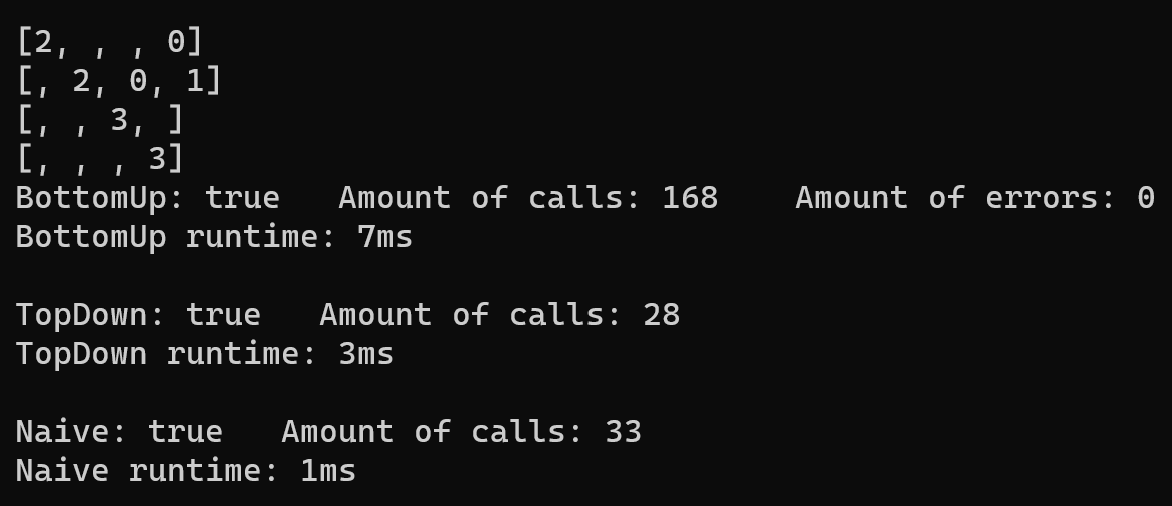
\includegraphics[scale=0.6]{images/terminal_2.png}
\end{minipage}\begin{minipage}{0.6\textwidth}
Then the results, counter and runtime in $ms$ is shown for each parsing method. \\
For the \texttt{BottomUp} method is the CYK algorithm table printed.
\end{minipage}









%---------------------------------------------------------------------%








\section{Graphs and additional results}
\label{previousresults}


The following tables show some tests that were run with the different parsing methods and grammars. The first of each column for the method shows the truth value that is returned (as T for true and F for false), C represents the counter and T the time in ms. Those tests were run before the BottomUp method was working correctly.
\\
\\
\\
\\
Well-Balanced-Parantheses: \\
\\
\begin{tabular}{|c|c||c|c|c||c|c|c||c|c|c|}
\hline
Word & Length & N & NC & NT & B & BC & BT & T & TC & TT \\
\hline
\hline
() & 2 & T & 6 & 5ms & F & 0 & 2ms & T & 6 & 1ms \\
\hline
(()) & 4 & T & 33 & 4ms & F & 84 & 3ms & T & 28 & 1ms \\
\hline
((())) & 6 & T & 212 & 6ms & F & 360 & 6ms & T & 84 & 1ms \\
\hline
(((()))) & 8 & T & 1295 & 6ms & F & 924 & 9ms & T & 190 & 1ms \\
\hline
((((())))) & 10 & T & 7666 & 9ms & F & 1872 & 11ms & T & 362 & 1ms \\
\hline
(((((((((()))))))))) & 20 & T & 51.863.993 & 1049ms & F & 15.732 & 23ms & T & 2.772 & 3ms \\
\hline
((...)) & 40 & & & & F & 127.452 & 50ms & T & 21.743 & 4ms \\
\hline
\end{tabular}

\ \\
The input word with a length of 40 did not terminate for the naive parsing in 60 minutes.
\\
\\
\\
\\
Stupid Grammar:\\
\\
\begin{tabular}{|c|c||c|c|c||c|c|c||c|c|c|}
\hline
Word & Length & N & NC & NT & B & BC & BT & T & TC & TT \\
\hline
\hline
aaaa & 4 & F & 33 & 5ms & F & 28 & 6ms & F &27 & 1ms \\
\hline
aaaaaaaa & 8 & F & 1.596 & 8ms & F & 308 & 5ms & F & 197 & 1ms \\
\hline
aaaaaaaaaaaaaaaa & 16 & F & 3.524.577 & 89ms & F & 2.660 & 15ms & F & 1.481 & 1ms \\
\hline
\end{tabular}


\subsection*{Graphs:}
\label{graph}
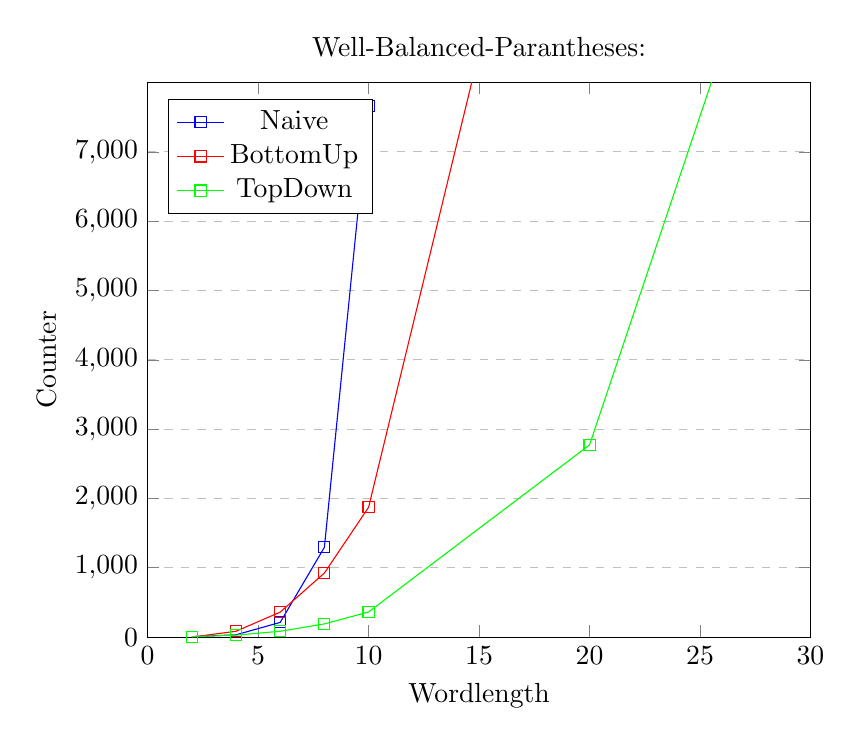
\begin{tikzpicture}
\begin{axis}[
    title={Well-Balanced-Parantheses:},
    xlabel={Wordlength},
    ylabel={Counter},
    xmin=0, xmax=30,
    ymin=0, ymax=8000,
    xtick={0,5,10,15,20,25,30},
    ytick={0, 1000,2000,3000,4000,5000, 6000, 7000},
    legend pos=north west,
    ymajorgrids=true,
    grid style=dashed,
]

\addplot[
    color=blue,
    mark=square,
    ]
    coordinates {
    (2,6)(4, 33)(6, 212)(8, 1295)(10, 7666)
    };

    
\addplot[
    color=red,
    mark=square,
    ]
    coordinates {
    (2,0)(4, 84)(6, 360)(8, 924)(10, 1872)(20,15000)
    };

    
\addplot[
    color=green,
    mark=square,
    ]
    coordinates {
    (2,6)(4, 28)(6, 84)(8, 190)(10, 362)(20,2772)(40, 21742)
    };
    \legend{Naive, BottomUp, TopDown}
    
\end{axis}
\end{tikzpicture}

\ \\

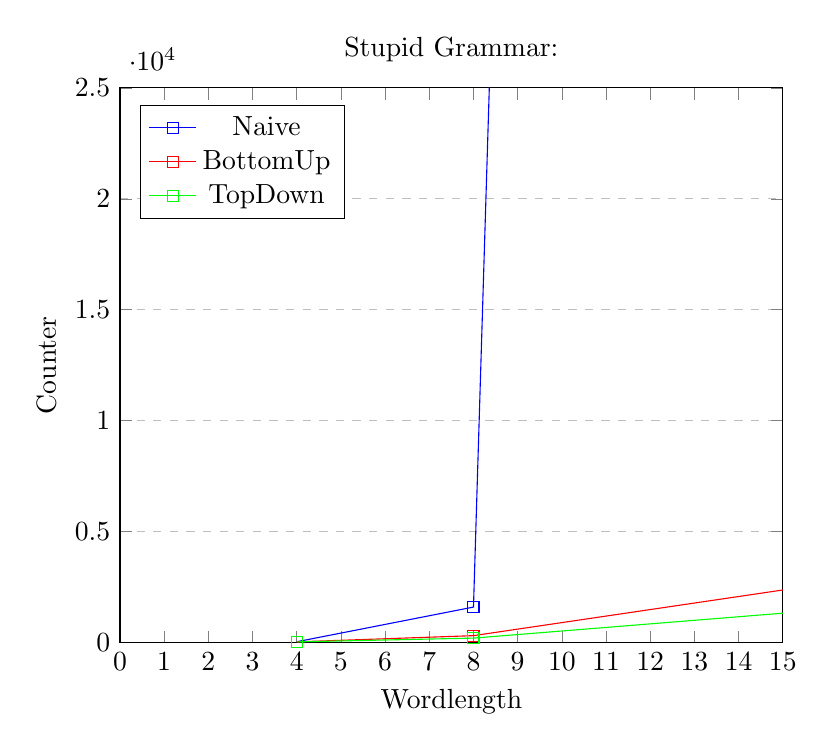
\begin{tikzpicture}
\begin{axis}[
    title={Stupid Grammar:},
    xlabel={Wordlength},
    ylabel={Counter},
    xmin=0, xmax=15,
    ymin=0, ymax=25000,
    xtick={0,1,2,3,4,5,6,7,8,9,10,11,12,13,14,15},
    ytick={0, 5000,10000,15000,20000,25000},
    legend pos=north west,
    ymajorgrids=true,
    grid style=dashed,
]

\addplot[
    color=blue,
    mark=square,
    ]
    coordinates {
    (4,33)(8, 1596)(16, 524577)
    };

    
\addplot[
    color=red,
    mark=square,
    ]
    coordinates {
    (4,28)(8, 308)(16, 2660)
    };

    
\addplot[
    color=green,
    mark=square,
    ]
    coordinates {
    (4,27)(8, 197)(16, 1481)
    };
    \legend{Naive, BottomUp, TopDown}
    
\end{axis}
\end{tikzpicture}










%---------------------------------------------------------------------%







\newpage
\section{Calculations}

\subsection{CNF Algorithm on an example}
\label{createcnf}

In this part, the following ruleset of a grammar will be translated into \textit{CNF}.

\begin{align*}
\texttt{S} & \rightarrow \texttt{SS} \mid  \texttt{aSb} \mid \texttt{ab} 
\end{align*}

\begin{enumerate}

\item Remove every nonterminal symbol that cannot be reached or is not generating another symbol: \\
\texttt{S} is the only nonterminal symbol and does not need to be removed.

\item Remove all symbols that cannot be reached. (All symbols can be reached.)

\item Replace the terminal symbols in the body of other rules with new nonterminal symbols to not have bodies which contain terminal and nonterminal symbols:
\begin{align*}
\texttt{S} & \rightarrow \texttt{SS} \mid  \texttt{LSR} \mid \texttt{LR}  \\
\texttt{L} & \rightarrow \texttt{a} \\
\texttt{R} & \rightarrow \texttt{b} 
\end{align*}


\item On the right side of the rules are only two nonterminal symbols allowed:
\begin{align*}
\texttt{S} & \rightarrow \texttt{SS} \mid  \texttt{LA} \mid \texttt{LR}  \\
\texttt{A} & \rightarrow \texttt{SR} \\
\texttt{L} & \rightarrow \texttt{a} \\
\texttt{R} & \rightarrow \texttt{b} 
\end{align*}

\item Remove all $\epsilon$-rules and paste in the start symbol what can be generated by them. (This grammar does not have $\epsilon$-rules.)

\item Check on transitivity and remove those dependencies. (There are no transitive rules here.)

\end{enumerate}

This is the grammar in CNF:
\begin{align*}
\texttt{S} & \rightarrow \texttt{SS} \mid  \texttt{LA} \mid \texttt{LR}  \\
\texttt{A} & \rightarrow \texttt{SR} \\
\texttt{L} & \rightarrow \texttt{a} \\
\texttt{R} & \rightarrow \texttt{b} 
\end{align*}


%---------------------------------------------------------------------%

\newpage

\subsection{CYK Algorithm on an example}
\label{cyksteps}

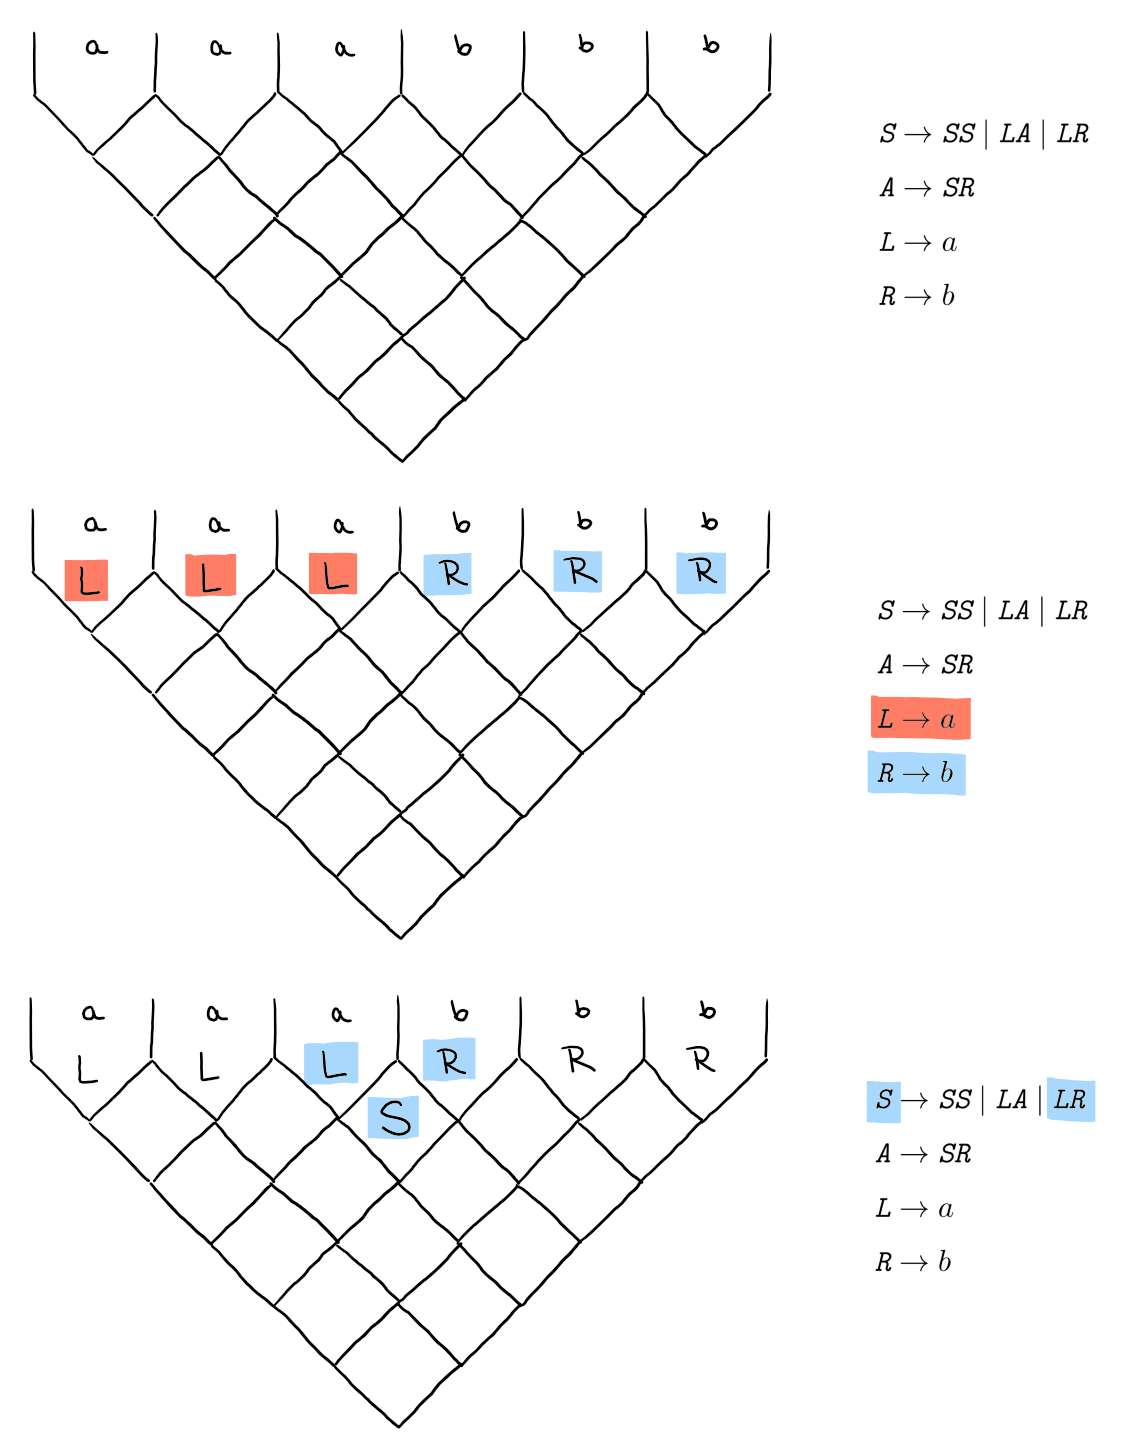
\includegraphics[scale=0.45]{images/cyk1.png}

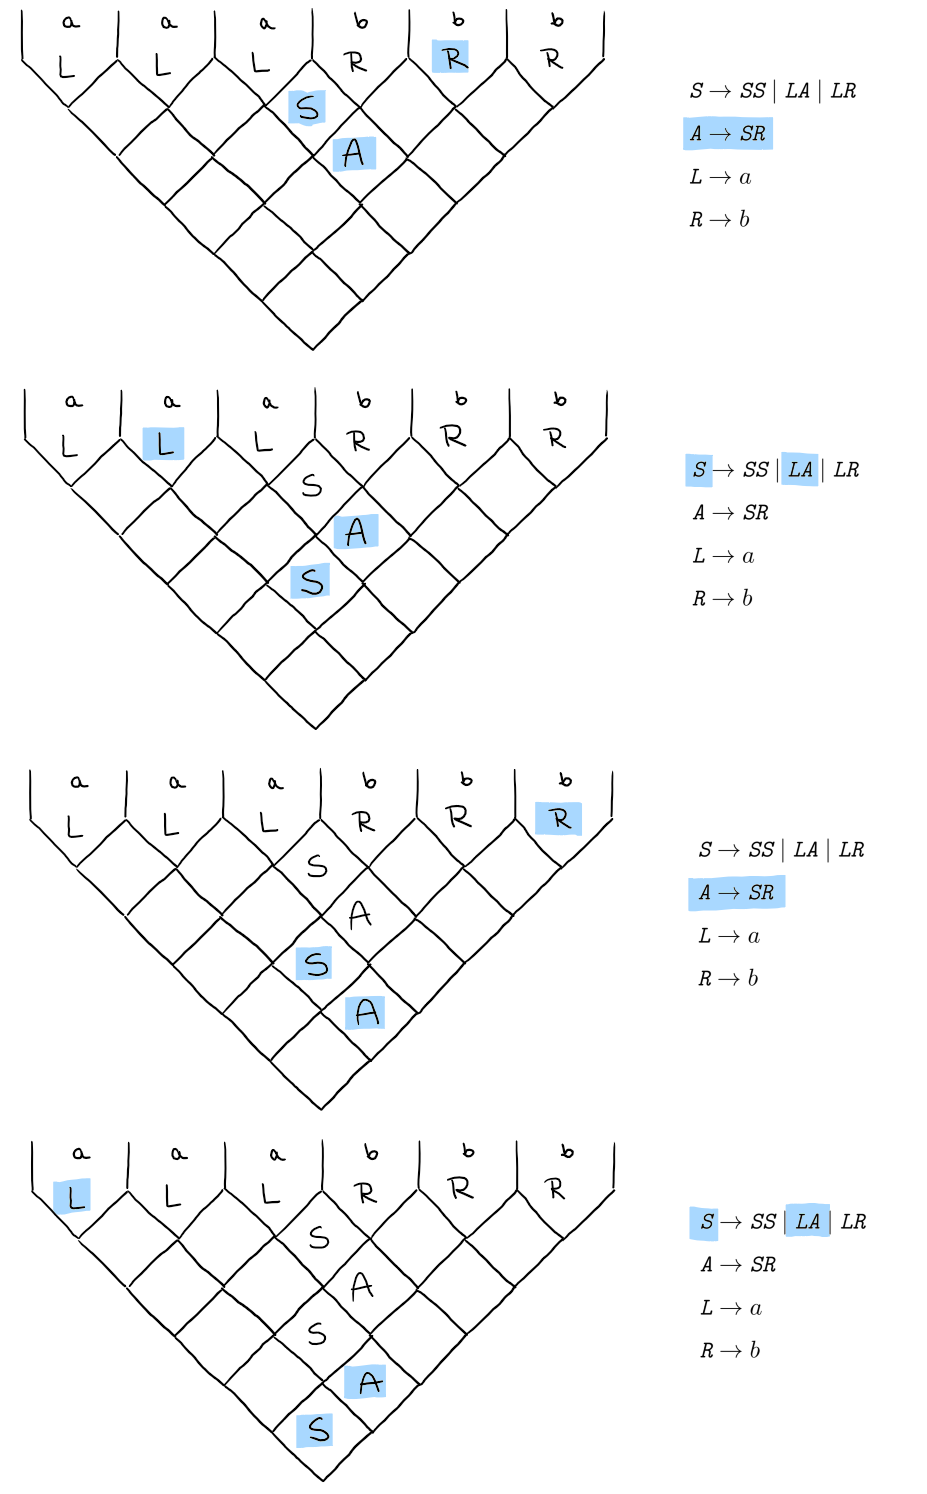
\includegraphics[scale=0.55]{images/cyk2.png}





%---------------------------------------------------------------------%
\fancyhead[LO]{\empty}




\newpage
\phantomsection
\addcontentsline{toc}{section}{\bibname}
%\begin{spacing}{1.3}
\printbibliography
%\end{spacing}



\end{document}